\chapter{Hardware}
\label{cha:hardware}

\section*{Prototyp-Aufbau}

Zur Entwicklung und Validierung der Firmware sowie zur Verifikation der Sensorintegration wurde ein vollständig funktionsfähiger Prototyp auf Basis des \textbf{Seeed Studio Wio-E5 Mini}-Entwicklungsboards aufgebaut. Das Wio-E5 Mini integriert einen STM32WLE5JC (inklusive Sub-GHz-LoRa-Transceiver) auf einem kompakten Formfaktor mit Stiftleisten und einer integrierten USB-UART-Bridge. Dadurch eignet es sich ideal für das schnelle Prototyping von LoRaWAN-Endknoten, ohne dass ein externer Programmierer oder eine eigene Spannungsversorgungsschaltung nötig ist.

Die sechs Sensoren des Referenzdesigns wurden als fertige \textbf{Breakout-Boards} beschafft – fünf davon von Adafruit, das SCD41-Breakout von Seeed Studio. Alle Breakouts sind über Jumperwires mit dem Wio-E5 Mini verbunden; der gesamte Aufbau erfolgte auf einem Steckbrett. Dies ermöglicht ein schnelles Tauschen von Sensoren und Anpassen der Beschaltung ohne Lötarbeiten. Alle sechs Sensoren wurden im Prototyp erfolgreich in Betrieb genommen und die vollständige Firmware verifiziert.

Der I2C-Bus des Prototyps entspricht dem des finalen Custom~PCBs: alle Sensoren hängen am selben I2C2-Bus (SDA: PA15, SCL: PB15) mit $4{,}7\,\text{k}\Omega$-Pull-up-Widerständen gegen VDD. Die Firmware unterscheidet zwischen Prototyp und Custom-PCB ausschließlich über den CMake-Build-Type (\texttt{Debug} für das Wio-E5, \texttt{Release} für das Custom-PCB), da der STM32WL55 im Wio-E5 dem STM32WLE5CCU6 im Custom-PCB hardwaretechnisch sehr ähnlich ist.

\begin{table}[H]
  \centering
  \begin{tabular}{lllll}
    \hline
    \textbf{Sensor} & \textbf{Hersteller} & \textbf{Messgrößen} & \textbf{I2C-Addr.} & \textbf{Breakout von} \\
    \hline
    SHT45    & Sensirion & Temperatur, Luftfeuchte & 0x44 & Adafruit \\
    BMP390   & Bosch     & Luftdruck               & 0x77 & Adafruit \\
    LTR390   & Lite-On   & UV-Licht, Umgebungslicht & 0x53 & Adafruit \\
    SCD41    & Sensirion & CO\textsubscript{2}-Konzentration & 0x62 & Seeed Studio \\
    SPS30    & Sensirion & Feinstaub (PM/NC)        & 0x69 & Sensirion \\
    MAX17048 & Maxim     & Akkuspannung             & 0x36 & Adafruit \\
    \hline
  \end{tabular}
  \caption{Sensoren und Breakout-Boards im Prototyp}
  \label{tab:breakouts}
\end{table}

Die Breakout-Boards eignen sich nicht nur zum Prototyping, sondern können auch direkt in kleinen Forschungsaufbauten eingesetzt werden. Im finalen Custom PCB sind dieselben Sensorchips als bare-die-Bauteile bestückt; lediglich die Beschaltung und das Layout sind optimiert.

\newpage

\section*{Sensoren im Detail}

\subsection*{Temperatur und relative Luftfeuchte: Sensirion SHT45}

Der SHT45 ist ein hochpräziser digitaler Temperatur- und Feuchtigkeitssensor von Sensirion. Im \textit{Single-Shot High Repeatability}-Modus liefert er Messwerte mit einer Genauigkeit von $\pm 0{,}1\,{^\circ}$C (Temperatur) und $\pm 1{,}0\,\%\text{rH}$ (relative Feuchte) bei einer Messzeit von ca.\ $8{,}3\,\text{ms}$. Die I2C-Adresse lautet \texttt{0x44}.

\subsection*{Luftdruck: Bosch BMP390}

Der BMP390 ist ein barometrischer Drucksensor mit einer absoluten Genauigkeit von $\pm 0{,}5\,\text{hPa}$ und einer relativen Genauigkeit von $\pm 0{,}03\,\text{hPa}$. Die Firmware nutzt den \textit{Forced Mode}: Der Sensor führt auf Befehl eine einzelne Messung durch ($\approx 2\,\text{ms}$ bei $720\,\mu\text{A}$) und wechselt danach automatisch in den Sleep-Modus ($2\,\mu\text{A}$). Die I2C-Adresse beträgt \texttt{0x77}.

\subsection*{UV-Licht: Lite-On LTR390}

Der LTR390 misst ultraviolettes Licht (UVA) sowie Umgebungslicht (ALS) in zwei separat auswählbaren Modi. Die Firmware berechnet daraus den UV-Index (UVI) direkt in Hardware. Die I2C-Adresse lautet \texttt{0x53}.

\subsection*{CO\textsubscript{2}-Konzentration: Sensirion SCD41}

Der SCD41 ist ein kompakter photoacoustischer CO\textsubscript{2}-Sensor mit einer Messgenauigkeit von $\pm 40\,\text{ppm}$ im Bereich 400–2000~ppm. Er nutzt das \textit{Single-Shot}-Messprinzip: Auf Befehl startet er eine einzige Messung, die ca.\ 5~Sekunden dauert, und wechselt danach automatisch in den Power-Down-Zustand ($\approx 0\,\mu\text{A}$). Eine CO\textsubscript{2}-Messung verbraucht eine Ladung von $q_{ss} = 77\,\text{mC}$, was den SCD41 zum energetisch dominantesten Sensor im System macht (s.\ Kapitel~\ref{cha:energie}). Die I2C-Adresse lautet \texttt{0x62}. Das Breakout-Board stammt von Seeed Studio.

\subsection*{Feinstaub: Sensirion SPS30}

Der SPS30 misst Partikelmassenkonzentration (PM1.0, PM2.5, PM4.0, PM10.0) sowie Partikelzahlkonzentration (NC0.5 bis NC10.0) und die typische Partikelgröße mittels Laserstreulichtmessung und einem internen Gebläse. Er benötigt eine 5-V-Versorgungsspannung für den Lüfter. Da der Gebläsebetrieb energieintensiv ist, wird der SPS30 durch die Firmware nur alle 30~Minuten aktiviert und danach sofort wieder in den Sleep-Modus versetzt. Eine automatische Lüfterreinigung (\textit{Fan Cleaning}) wird nach je 120~Stunden Betrieb oder per Downlink-Befehl ausgelöst, um Ablagerungen auf dem optischen Sensor zu verhindern. Die I2C-Adresse lautet \texttt{0x69}.

\subsection*{Akkuzustand: Maxim MAX17048}

Der MAX17048 ist ein Fuel-Gauge-IC, der die Zellenspannung des LiPo-Akkus über I2C bereitstellt. Die Firmware nutzt ausschließlich die Spannungsmessung in~mV, um den Ladezustand abzuschätzen und das Sendeverhalten entsprechend anzupassen. Der Ruhestrom des MAX17048 beträgt $1{,}5\,\mu\text{A}$; eine Leseoperation dauert wenige Millisekunden bei $\approx 500\,\mu\text{A}$. Die I2C-Adresse ist \texttt{0x36}.

\newpage

\section*{Spannungsversorgung}

\subsection*{Prototyp}

Im Steckbrett-Prototyp werden zwei separate Spannungsregler eingesetzt:

\begin{itemize}
  \item \textbf{TPS63900 (Texas Instruments):} Buck-Boost-Konverter, erzeugt $3{,}3\,\text{V}$ aus der LiPo-Batterie ($2{,}5$–$4{,}2\,\text{V}$). Mit einem Quiescent Current von $<0{,}5\,\mu\text{A}$ bei über $95\,\%$ Effizienz ist er ideal für Ultra-Low-Power-Anwendungen.
  \item \textbf{Pololu Step-Up-Konverter:} Hebt $2{,}3$–$4{,}8\,\text{V}$ auf $5\,\text{V}$ für den SPS30 an. Dieser Konverter hat jedoch einen Quiescent Current von ca.\ $400\,\mu\text{A}$ — das ist mehr als der gesamte theoretische Ruhestrom des finalen Systems.
\end{itemize}

Der hohe Quiescent Current des Pololu-Moduls dominiert den Gesamtstromverbrauch des Prototyps im Sleep-Modus und ist der Hauptgrund, warum die Strommessungen am Prototyp deutlich über dem theoretischen Wert liegen (s.\ Kapitel~\ref{cha:energie}).

\subsection*{Custom PCB}

Im finalen PCB-Design werden zwei \textbf{TPS63900}-Konverter eingesetzt:

\begin{itemize}
  \item \textbf{TPS63900 (Primär):} $3{,}3\,\text{V}$ Systemversorgung (STM32WLE5, alle I2C-Sensoren außer SPS30).
  \item \textbf{TPS63900 (Sekundär):} $5\,\text{V}$ Versorgung für den SPS30. Wird über einen GPIO-Pin des STM32 softwaregesteuert aktiviert und kann alternativ via Jumper permanent eingeschaltet werden. Mit einem Wirkungsgrad von $>95\,\%$ und einem Quiescent Current von $<0{,}5\,\mu\text{A}$ im Ruhezustand stellt dieser Regler auch im Dauerbetrieb keinen nennenswerten Energieverbrauch dar.
\end{itemize}

Den Solar-MPPT-Lader übernimmt der \textbf{BQ25185} (Texas Instruments): Er verwaltet die Energiegewinnung aus einem kleinen Solarmodul und lädt den Einzelzellen-LiPo-Akku. Damit ist das System vollständig autark betreibbar.

\begin{table}[H]
  \centering
  \begin{tabular}{llll}
    \hline
    \textbf{Komponente} & \textbf{Aufgabe} & \textbf{Quiescent Current} & \textbf{Eingesetzt} \\
    \hline
    TPS63900 (Primär) & $3{,}3\,\text{V}$ aus LiPo  & $< 0{,}5\,\mu\text{A}$ & Prototyp + PCB \\
    TPS63900 (Sekundär) & $5\,\text{V}$ aus LiPo & $< 0{,}5\,\mu\text{A}$ & Nur PCB \\
    BQ25185 & Solar-MPPT-Laden & $\approx 1\,\mu\text{A}$ (inaktiv) & Nur PCB \\
    Pololu Step-Up & $5\,\text{V}$ aus LiPo & $\approx 400\,\mu\text{A}$ & Nur Prototyp \\
    \hline
  \end{tabular}
  \caption{Spannungsregler im Vergleich: Prototyp vs.\ Custom PCB}
  \label{tab:regler}
\end{table}

\newpage

\section*{PCB-Design}

\subsection*{Übersicht}

Die Leiterplatte wurde vollständig in \textbf{EasyEDA Pro} designed. Es handelt sich um ein \textbf{4-lagiges PCB} mit dedizierten Lagen für Signal, Masse, Versorgung und weiteres Signal. Die 4-Lagen-Technologie ermöglicht eine durchgehende Massefläche unter allen kritischen Signalpfaden, was insbesondere für das RF-Layout entscheidend ist.

Das Herzstück der Platine bildet der \textbf{STM32WLE5CCU6} (UFQFPN48) — ein System-on-Chip, der einen ARM Cortex-M4 mit 48~MHz und einem integrierten Sub-GHz-LoRa-Transceiver kombiniert. Im Gegensatz zu modularen LoRaWAN-Lösungen (fertigen Modulen) ermöglicht der direkte Einsatz des bare-die-Chips vollständige Kontrolle über das RF-Frontend-Layout und eliminiert die Kostenaufschläge fertiger Module.

\subsection*{RF-Frontend-Layout}

Das RF-Layout des STM32WLE5 erfordert besondere Sorgfalt, da der integrierte Sub-GHz-Transceiver direkt an der PCB-Antenne betrieben wird. Folgende RF-Komponenten sind auf dem Custom-PCB verbaut:

\begin{itemize}
  \item \textbf{BALFHB-WL-02D3 (Johanson Technology):} Balun für die Impedanzanpassung zwischen dem differenziellen RF-Ausgang des STM32WLE5 und dem $50\,\Omega$-Antennenanschluss.
  \item \textbf{BGS12SN6 (Infineon):} RF-Schalter zur Umschaltung zwischen TX- und RX-Pfad. Wird durch einen einzigen GPIO-Pin (PC13) gesteuert.
\end{itemize}

Die Zuleitungen im RF-Pfad sind als Controlled-Impedance-Leiterbahnen ($50\,\Omega$) ausgeführt. Unter dem gesamten Antennen-Speisepfad liegt eine durchgehende Massefläche; Isolationsbereiche um den Chip-Antennensockel verhindern Einflüsse benachbarter Leiterbahnen.

\subsection*{Schaltplan}

\begin{figure}[H]
  \centering
  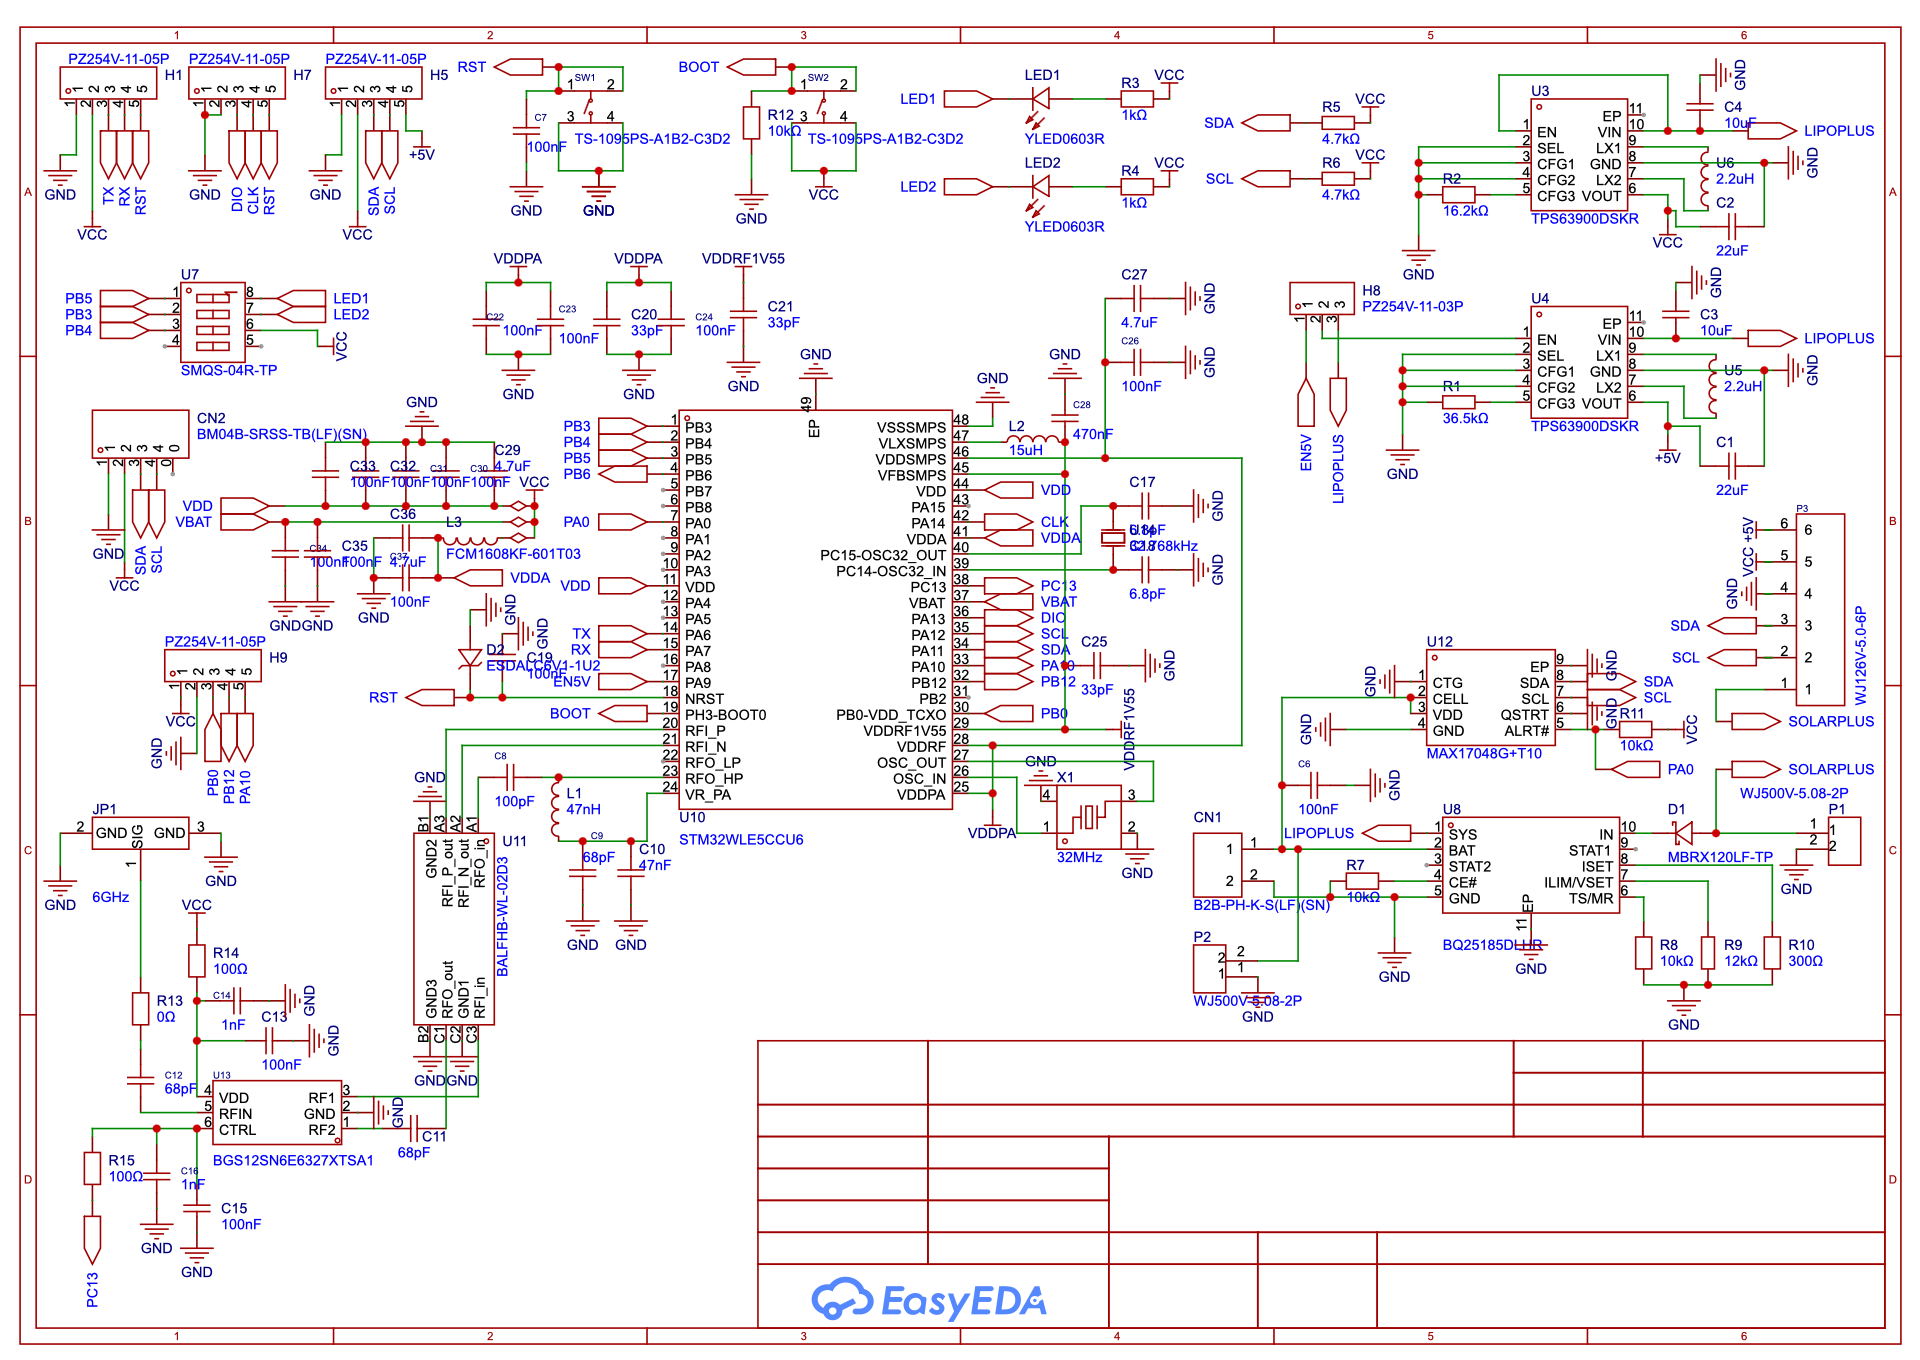
\includegraphics[width=\linewidth]{../../hardware/ordered_pcb/schematic_preview}
  \caption{Schaltplan der HydroNodeStation01 (EasyEDA Pro Render)}
  \label{fig:schematic}
\end{figure}

\newpage

\subsection*{PCB-Routing}

\begin{figure}[H]
  \centering
  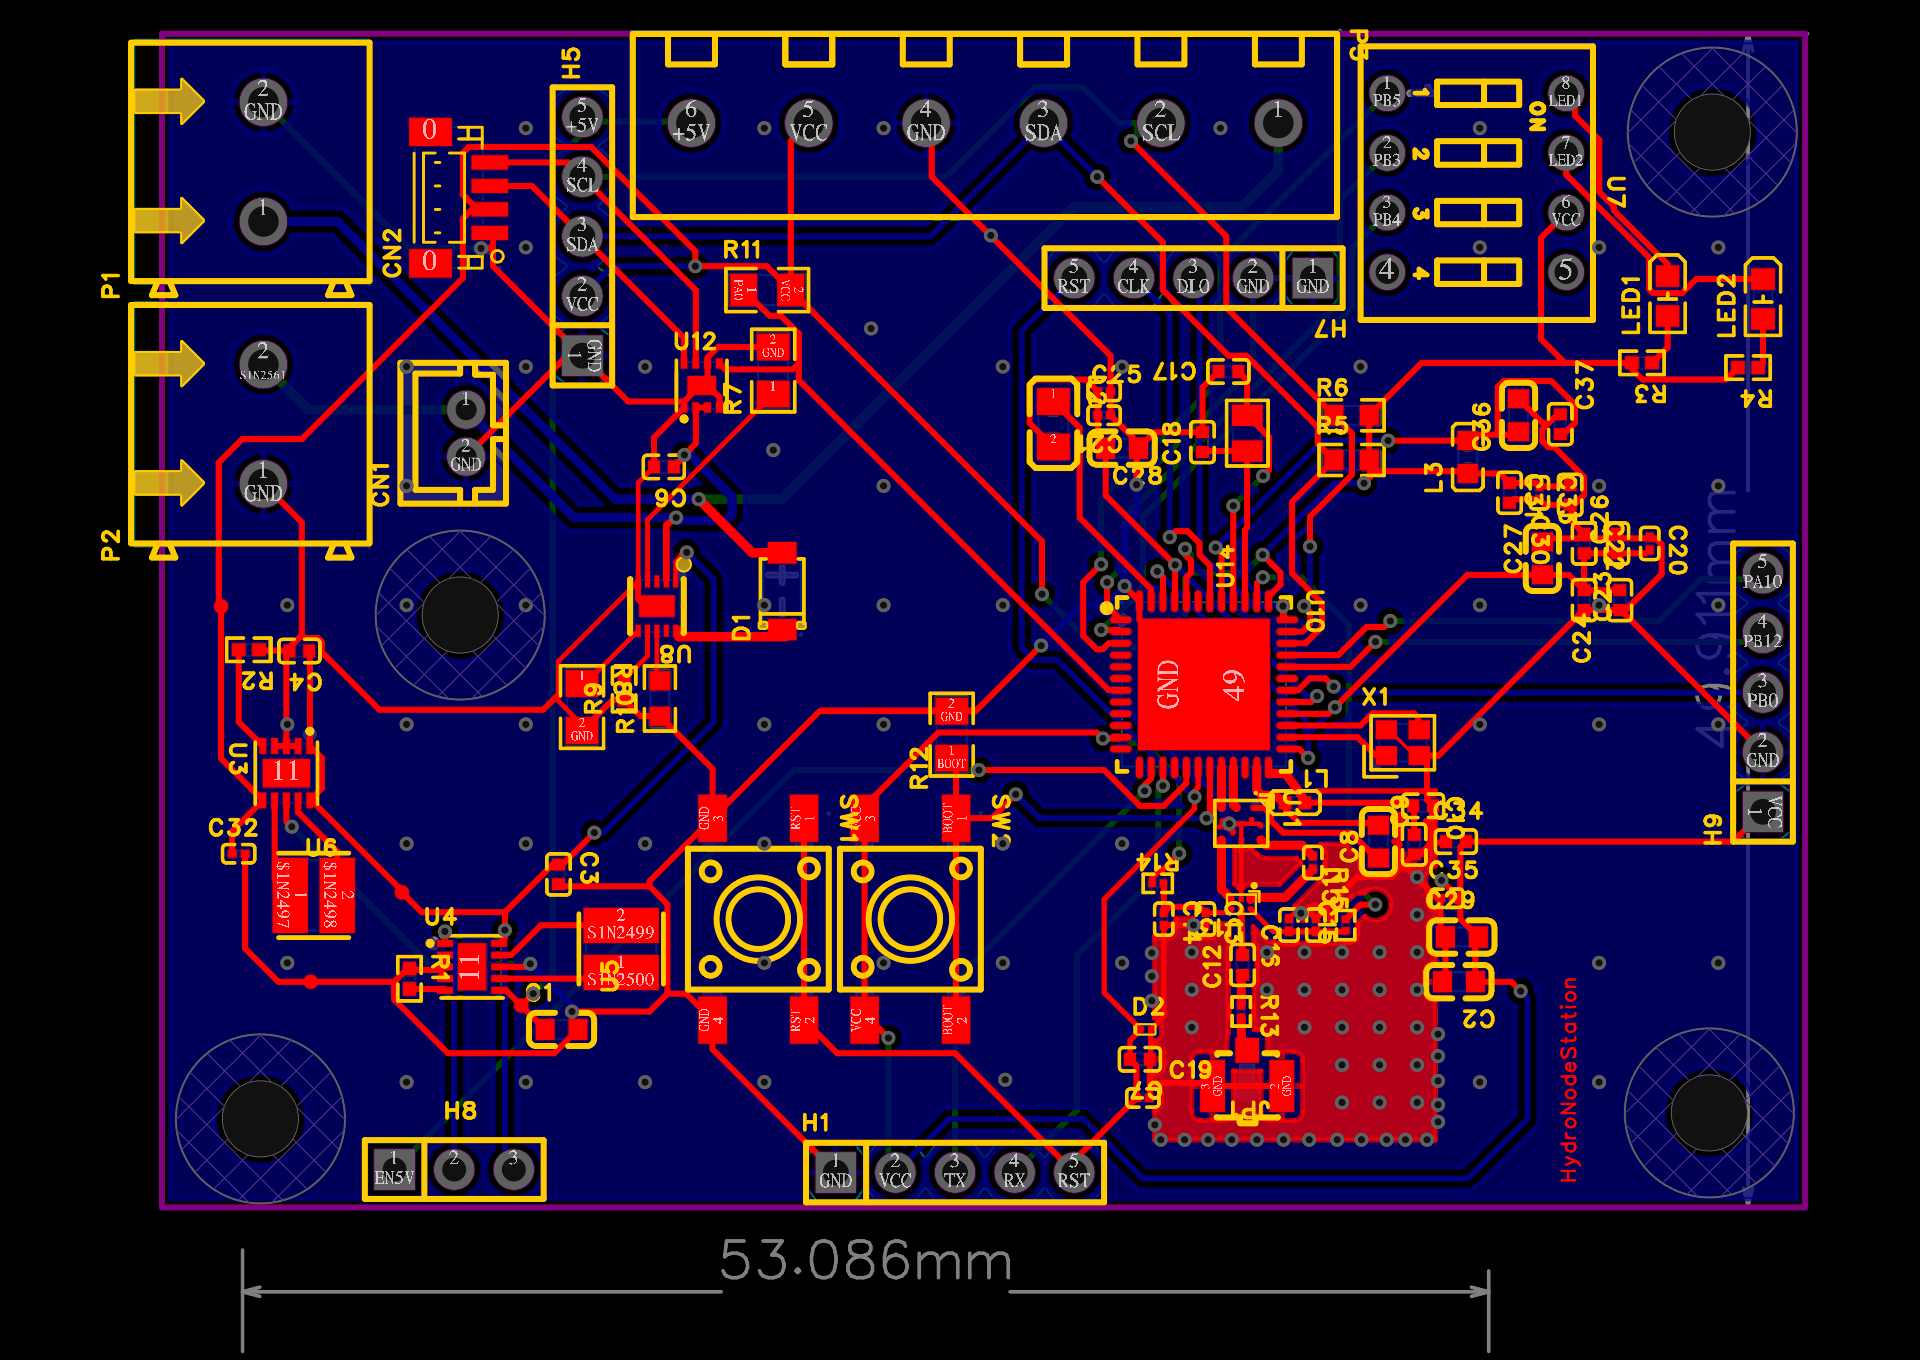
\includegraphics[width=0.88\linewidth]{../../hardware/ordered_pcb/pcb_routing}
  \caption{PCB-Layout mit Signallagen (EasyEDA Pro Render)}
  \label{fig:routing}
\end{figure}

\subsection*{3D-Ansicht}

\begin{figure}[H]
  \centering
  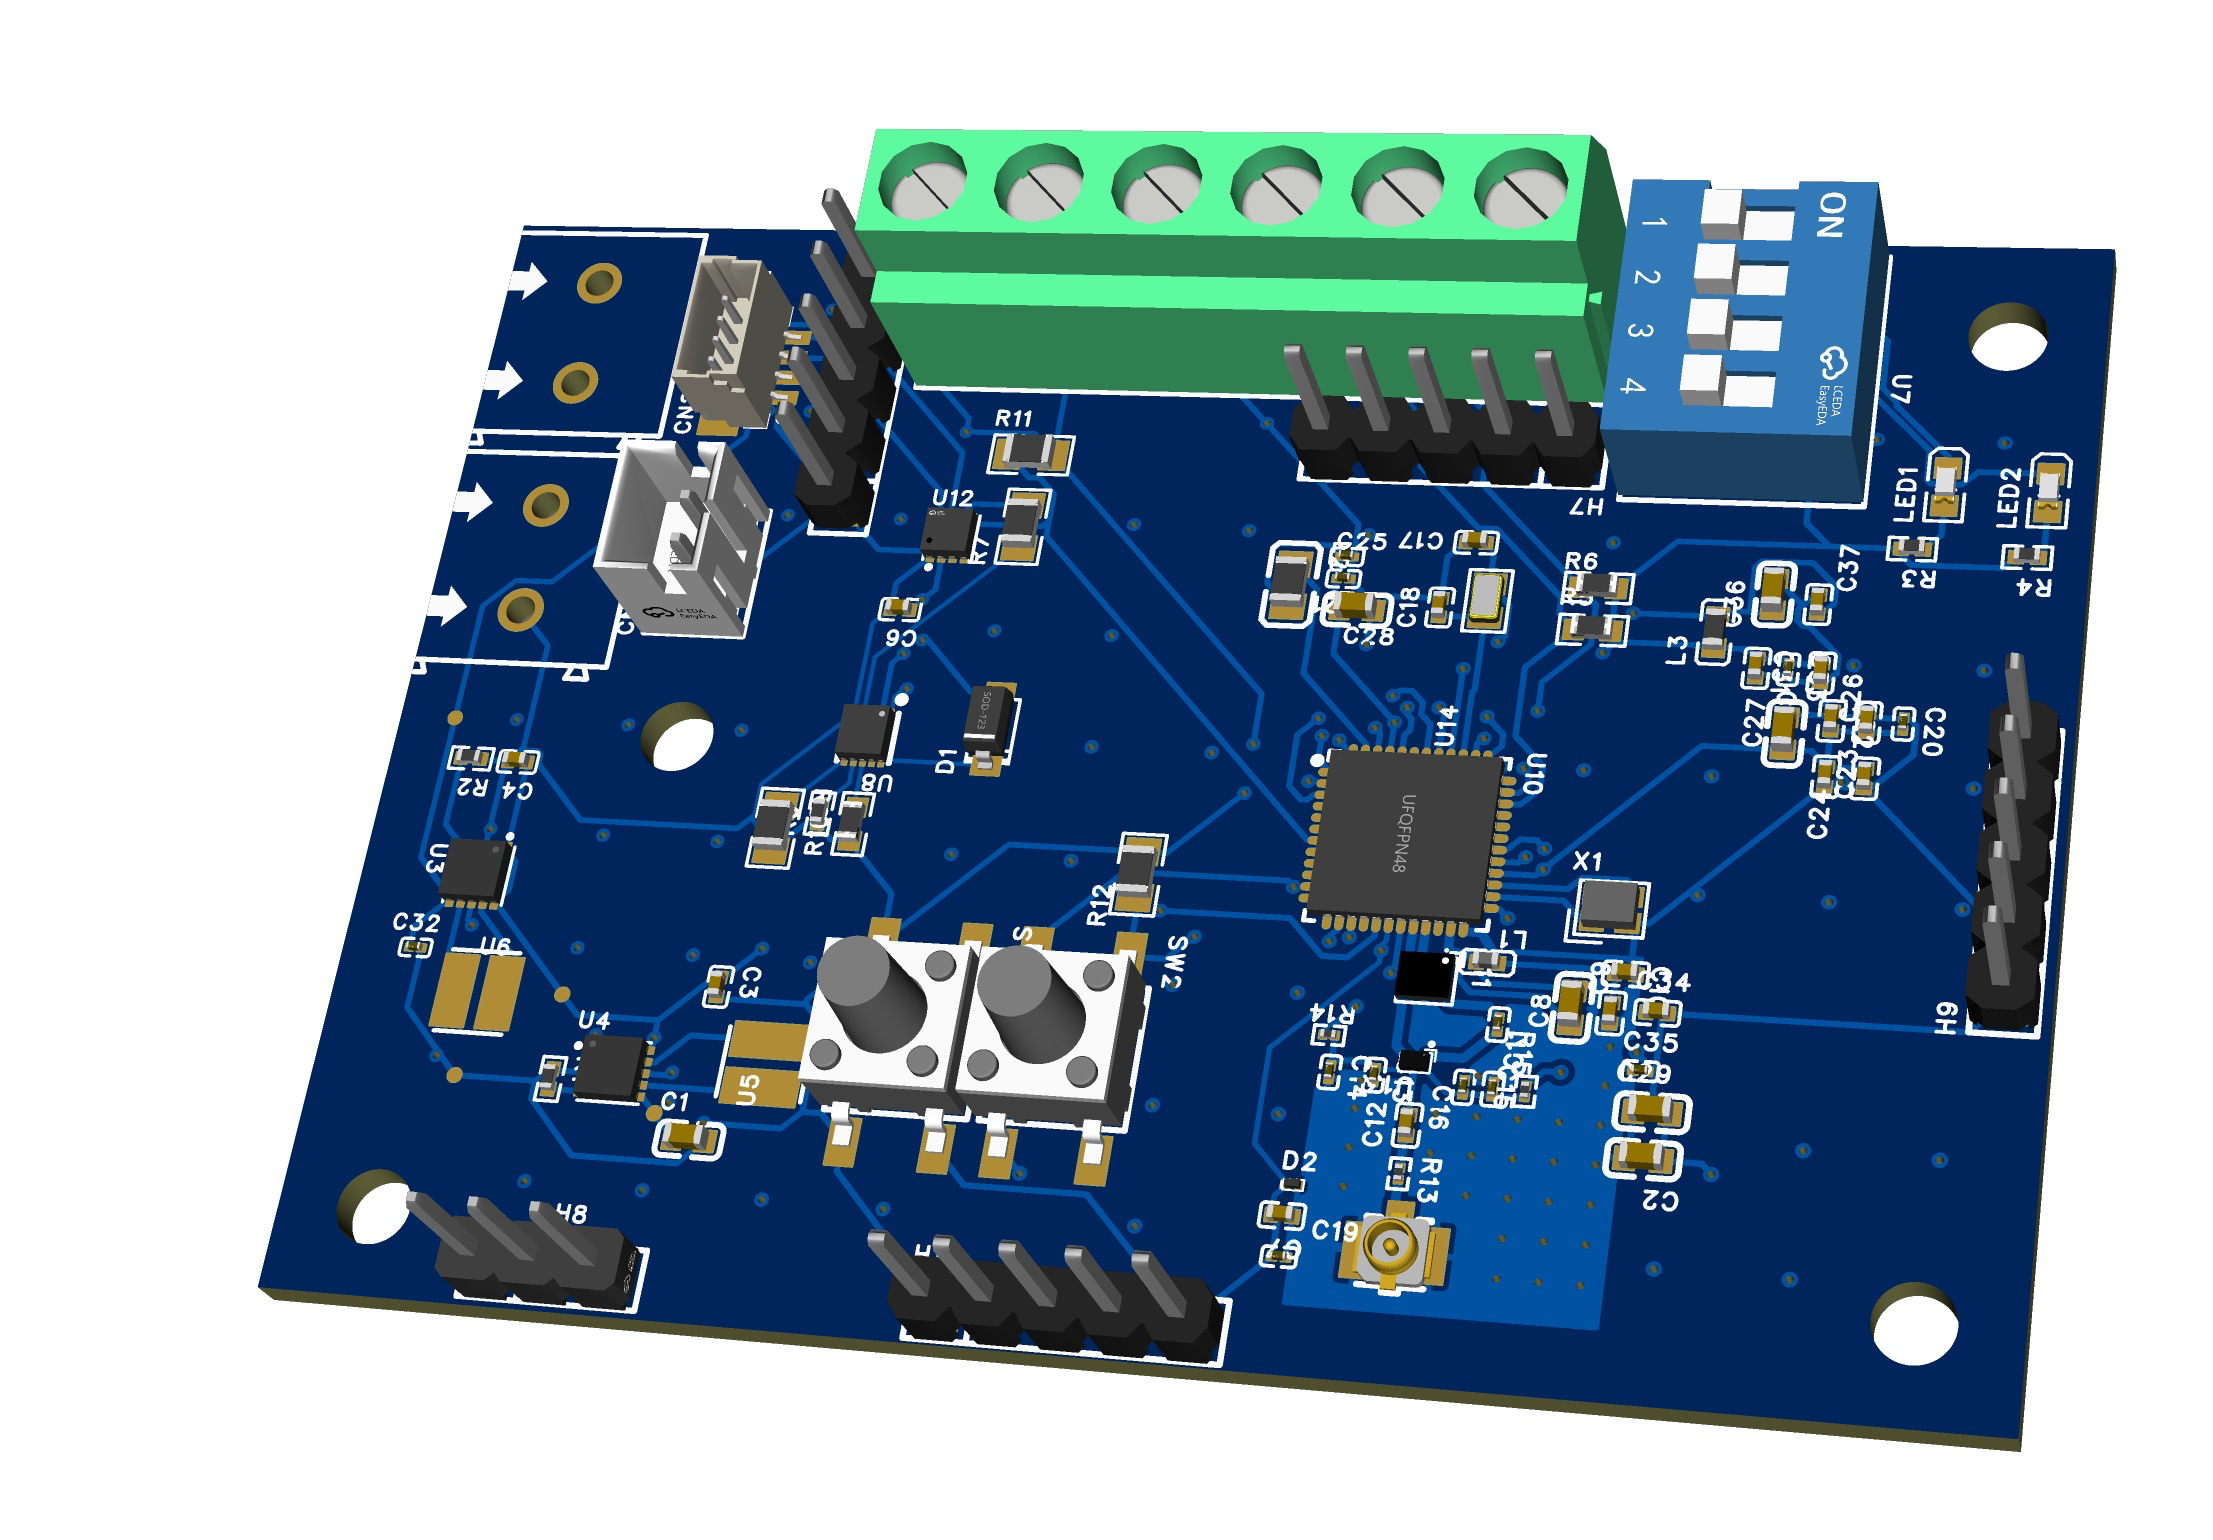
\includegraphics[width=0.72\linewidth]{../../hardware/ordered_pcb/pcb_3d_render}
  \caption{3D-Render des Custom PCB (EasyEDA Pro)}
  \label{fig:pcb3d}
\end{figure}

\newpage

\subsection*{Fertigung und Bestückung bei JLCPCB}

Die Leiterplatte wurde bei \textbf{JLCPCB} gefertigt und vollständig maschinell bestückt (PCBA — PCB Assembly). Die Bestellung umfasste:

\begin{itemize}
  \item \textbf{Anzahl:} 5 Platinen
  \item \textbf{Lagen:} 4
  \item \textbf{Lötstopplackfarbe:} Blau
  \item \textbf{Oberfläche:} HASL (bleifrei)
  \item \textbf{Bestückung:} Vollständig maschinell bestückt und verlötet (JLCPCB PCBA)
  \item \textbf{Gesamtkosten:} ca.\ 200\,€ inklusive Versand und Steuern
\end{itemize}

Ermöglicht wurde die Bestellung teilweise durch einen Gutschein im Wert von \textbf{150~USD}, den das Projekt im Rahmen des \textit{OSWHLAB Start 2026 Open Source Contest} erhalten hat (s.\ Kapitel~\ref{cha:opensource}). JLCPCB führt an bestückten Platinen standardmäßig visuelle Inspektion und Fliegende-Nadel-Tests durch; weiterführende Funktionstests werden nach Lieferung am eigenen Messplatz durchgeführt.

\section*{PCB-Überprüfung und Inbetriebnahme}
\label{sec:pcb-review}

Die Platinen wurden von JLCPCB geliefert und vollständig in Betrieb genommen. Im Folgenden sind die wichtigsten Ergebnisse dokumentiert.

\subsection*{TPS63900-Fehler und Workaround}

Bei der ersten Inbetriebnahme wurde festgestellt, dass der primäre TPS63900-Buck-Boost-Konverter für die 3,3-V-Systemversorgung nicht wie vorgesehen funktionierte. In Absprache mit einem Experten wurde der Fehler im PCB-Design identifiziert und analysiert. Als physischer Workaround wurde der fehlerhafte TPS63900 vom LiPo-Akku-Plus und dem 3,3-V-Netz getrennt. Derselbe Chip wurde auf einem Breakout-Board montiert und an die PCB-Header angesteckt. Das System läuft damit identisch wie vorgesehen, mit minimalem Overhead und gleicher Effizienz. Das korrigierte PCB-Design ist erarbeitet und für zukünftige Board-Revisionen bereit.

\subsection*{Sensor-Verifikation auf dem Custom PCB}

Alle fünf Kernsensoren wurden auf dem Custom PCB erfolgreich verifiziert. Sämtliche I2C-Kommunikation läuft stabil; die Messwerte sind plausibel und konsistent mit den Prototyp-Messungen. Der LoRaWAN-Stack verbindet sich zuverlässig über OTAA mit dem Helium-Netzwerk und sendet reguläre Uplinks auf allen drei konfigurierten Ports.

\subsection*{Strommessung mit dem PPK2}

Strommessungen mit dem Nordic Semiconductor Power Profiler Kit II (PPK2) wurden am Custom PCB durchgeführt (Messdatei: \texttt{ppk2-20260601T143444.ppk2}). Die Ergebnisse und Interpretation sind in Kapitel~\ref{cha:energie} dokumentiert.

\subsection*{Langzeit-Feldtest}

Die Station läuft seit Ende Mai 2026 im Außeneinsatz im 3D-gedruckten Stevenson-Screen-Gehäuse. Die Daten werden in Echtzeit über das Helium-Netzwerk übertragen und sind öffentlich einsehbar unter:\\
\url{https://hydronode.texhfexlabs.de/stations/public/004dd7e7-5c27-4de0-bff5-24116f721658}

Die bisherigen Feldtest-Ergebnisse sind positiv: alle Sensoren liefern stabile Werte, und der LoRaWAN-Uplink ist zuverlässig. Die vollständige Solar-Autarkie steht noch zur abschließenden Verifikation aus.

\section*{Gehäuse: Stevenson Screen}

Um die Sensoren vor direkter Sonneneinstrahlung und Niederschlag zu schützen, ohne die Luftzirkulation zu behindern, wird ein \textbf{Stevenson Screen} eingesetzt: eine klassische meteorologische Schutzeinhausung mit lamellierter Belüftung. Die weiße Außenfarbe reflektiert Sonnenstrahlung und verhindert übermäßige Erwärmung im Inneren. Für eine korrekte Messung von Außentemperatur und Luftfeuchtigkeit ist dies entscheidend: Ein Gehäuse, das sich durch direkte Sonneneinstrahlung aufheizt, würde verfälschte Temperaturwerte liefern.

Das Gehäuse wurde vollständig selbst in \textbf{Fusion 360} entworfen. Es besteht aus mehreren übereinandergesteckten Lamellenebenen, die direkte Sonneneinstrahlung und Regen blockieren, aber Luft frei zirkulieren lassen. Die Teile wurden aus weißem \textbf{ASA-Kunststoff} (Acrylnitril-Styrol-Acrylat) 3D-gedruckt. ASA ist UV-beständig und witterungsfest, was es für den Dauereinsatz im Außenbereich geeignet macht. Der Druck erfolgte auf einem eigens für das Projekt angeschafften 3D-Drucker. Mehrere Druckdurchläufe wurden benötigt, um Passgenauigkeit und Stabilität sicherzustellen.

Das Gehäuse ist montiert und befindet sich seit Ende Mai 2026 im Außeneinsatz. Die bisherigen Feldtest-Ergebnisse zeigen stabile Temperatur- und Feuchtemessungen ohne Überhitzungseffekte.

\begin{figure}[H]
  \centering
  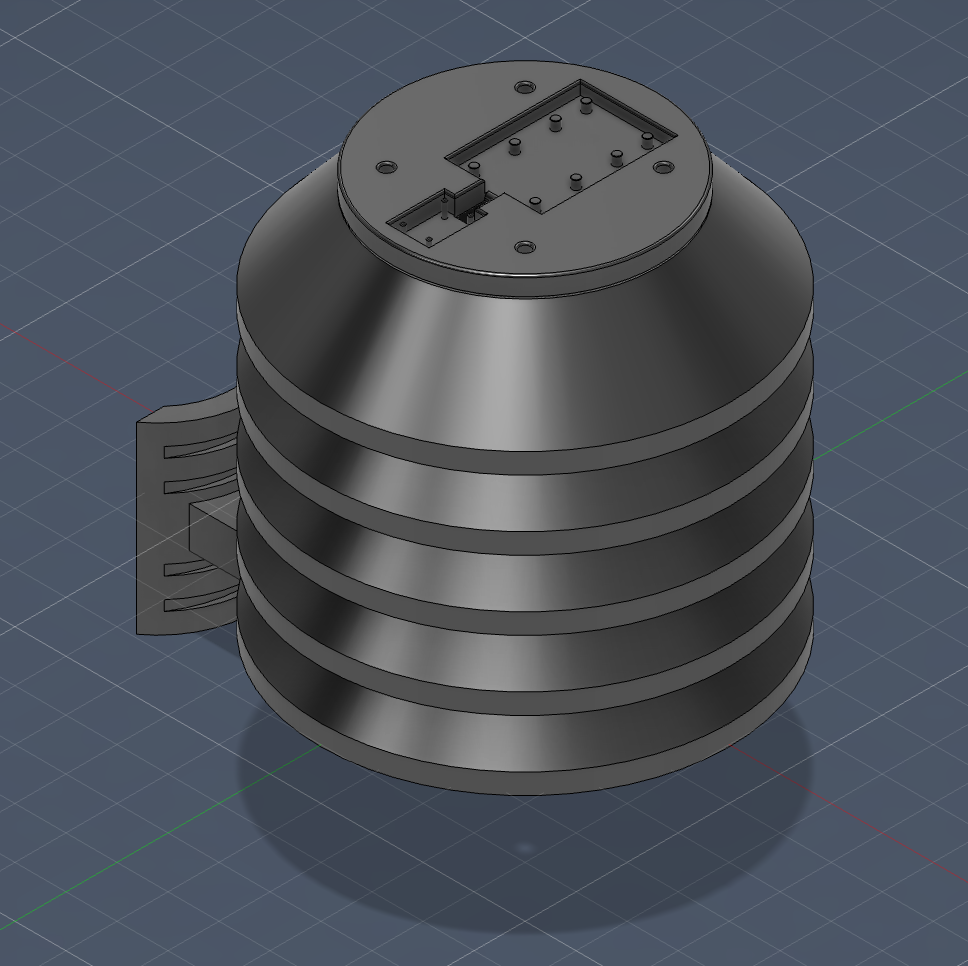
\includegraphics[width=0.6\linewidth]{../assets/stevenson_render}
  \caption{3D-Render des Stevenson-Screen-Gehäuses (Fusion 360)}
  \label{fig:stevenson-render}
\end{figure}

\begin{figure}[H]
  \centering
  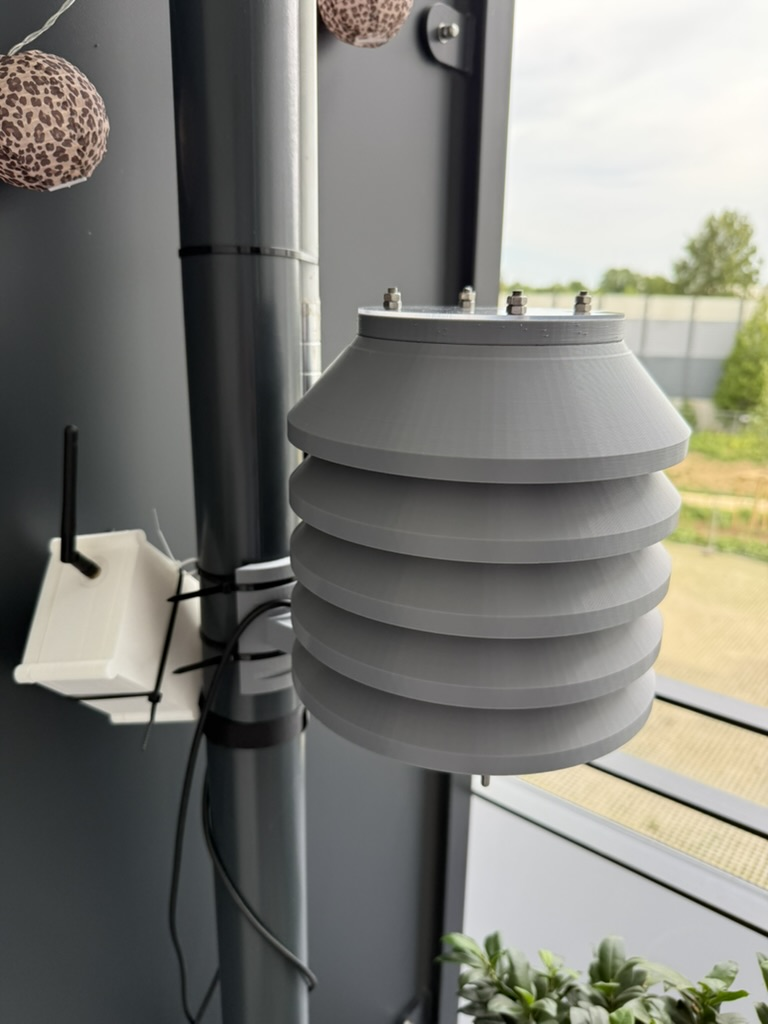
\includegraphics[width=0.6\linewidth]{../assets/station_outdoor}
  \caption{Montierte HydroNodeStation01 im Außeneinsatz}
  \label{fig:station-outdoor}
\end{figure}

\subsection*{UV-Sensorschutz: Acrylglas mit Korrekturfaktor}

Der LTR390-UV-Sensor benötigt eine Abdeckung, die ihn vor Schmutz und Niederschlag schützt, gleichzeitig aber UV-Licht transmittiert. UV-transparentes Spezialglas wäre ideal, ist jedoch kostenintensiv und schwer beschaffbar. Als kostengünstige Lösung wurde daher auf Standard-Acrylglas zurückgegriffen.

Eine Acrylglasplatte (ca.\ 2~mm Stärke) wurde mithilfe einer CNC-Maschine rund zugeschnitten, sodass sie passgenau in die vorgesehene Öffnung des Stevenson-Screen-Gehäuses eingesetzt werden kann.

Da Standard-Acrylglas einen Teil der UV-Strahlung absorbiert, wurde ein empirischer Korrekturfaktor ermittelt: Die Messstation nahm bei direkter Sonneneinstrahlung Messwerte mit und ohne Glasabdeckung auf und leitete aus dem Verhältnis einen Korrekturfaktor ab:

\begin{equation}
  \text{Korrekturfaktor} = \frac{\text{UVI}_\text{ohne Glas}}{\text{UVI}_\text{mit Glas}} = \frac{6{,}8}{5{,}2} = \frac{17}{13} \approx 1{,}31
\end{equation}

Dieser Faktor wird direkt in der Firmware als ganzzahlige Bruchrechnung angewandt (\texttt{uvi\_raw $\times$ 17 / 13}), um Fließkommaoperationen auf dem Mikrocontroller zu vermeiden. Die korrigierten UVI-Werte werden im Payload übertragen und im Backend direkt weiterverarbeitet.

Die STL-Dateien und Fusion-360-Quelldateien werden nach Abschluss des Feldtests zusammen mit den Hardware-Design-Dateien veröffentlicht (s.\ Kapitel~\ref{cha:opensource}).
